% Metódy inžinierskej práce

\documentclass[10pt,slovak,a4paper]{article}

\usepackage[slovak]{babel}
%\usepackage[T1]{fontenc}
\usepackage[IL2]{fontenc} % lepšia sadzba písmena Ľ než v T1
\usepackage[utf8]{inputenc}
\usepackage{graphicx}
\usepackage{url} % príkaz \url na formátovanie URL
\usepackage{hyperref} % odkazy v texte budú aktívne (pri niektorých triedach dokumentov spôsobuje posun textu)

\usepackage{cite}
%\usepackage{times}

\pagestyle{headings}

\title{Vývoj softvérových projektov v rámci Scrum\thanks{Semestrálny projekt v predmete Metódy inžinierskej práce, ak. rok 2020/21, vedenie: Ing. Vladimír Mlynarovič, PhD}} % meno a priezvisko vyučujúceho na cvičeniach

\author{Michal Darovec\\[2pt]
	{\small Slovenská technická univerzita v Bratislave}\\
	{\small Fakulta informatiky a informačných technológií}\\
	{\small \texttt{xdarovec@stuba.sk}}
	}

\date{\small 26. október 2021} % upravte



\begin{document}

\maketitle

\begin{abstract}
Cieľom tejto práce je predstaviť a bližšie ukázať spôsob vývoja softvérových projektov v rámci Scrum. V práci sa zoznámime s agilnou metodikou, v ktorej sa v súčasnosti robí veľké množstvo nielen softvérových projektov. Ďalej sa v práci zameriame priamo na Scrum, predstavíme si jeho princípy, pravidlá a filozofiu. Čitateľ bude oboznámený s problematikou Scrumu, rovnako s jeho výhodami a nevýhodami.

\textbf{Kľúčové slová:} agile, scrum, softvér, projekt, vývoj, inžinierstvo
\end{abstract}



\section{Úvod}

Agilná metodika je stále viac populárny spôsob vyvíjania softvérových projektov a väčšina efektívnych firiem ju v tejto dobe využíva. Ide o skupinu frameworkov, ktoré fungujú na princípe iteratívneho vývoja a na kolaborácii samostatne pracujúcich funkčných tímov.
Celá filozofia agilnej metodiky je zameraná na inováciu. Ľudia v dnešnej dobe pracujú vo vysoko dynamických prostrediach, kde inovácia je nevyhnutne potrebná pre úspešný vývoj produktu. Moderné technológie sa vyvíjajú tak rýchlo, že ak firma neaplikuje dynamický prístup, produkty môžu byť zastarané a prakticky nepoužiteľné.
Najznámejší framework agilnej metodiky je Scrum. Jeho cieľom je pomôcť ľuďom, tímom a organizáciám vytvárať hodnotu prostredníctvom prispôsobivého riešenia komplexných problémov. Scrum nie je detailne špecifikovaný, jeho pravidlá sú skôr na správne nasmerovanie a udržiavanie disciplíny v podniku. Ako uvádzajú hlavní vývojári tohto frameworku, Ken Schwaber a Jeff Sutherland: „Scrum je postavený na kolektívnej inteligencii ľudí, ktorí ho používajú.“~\cite{schwaber2020scrum}. K jeho hodnotám a filozofii sa dostaneme bližšie v časti~\ref{hodnoty}.
Scrum je hlavne založený na princípe rýchleho a efektívneho vývoja produktov, ktorý je v dnešnej dynamickej dobe kľúčový. Tieto dynamické princípy môžeme vidieť hlavne v svetových softvérových firmách. Scrum však nie je výhodné implementovať pri veľkom množstve rutinných a repetitívnych úloh, ako napríklad pri účtovníctve alebo predajných hovoroch. Aj keď s prechodom na Scrum prichádza veľké riziko, osvojuje si ho viac a viac progresívnych manažérov. Začína sa dokonca stále viac používať mimo sféry softvérového inžinierstva.


\section{Hodnoty a filozofia} \label{hodnoty}
Skôr, ako sa pustíme do jednotlivých častí tohto frameworku, ideme si opísať, na čom je Scrum vlastne postavený. Tvorcovia Scrumu sa inšpirovali empiristickou filozofiou, ktorej základné myšlienky sú, že vedomosti nadobúdame zo skúseností a rozhodnutia robíme na základe toho, čo máme preskúmané. Scrum je postavený aj na „lean thinking“, čo je metóda organizovania ľudských aktivít takým spôsobom, aby sa ľudia nemrhali časom a sústredili sa na to najdôležitejšie~\cite{schwaber2020scrum}. Už z filozofie môžeme pochopiť, na akých princípoch Scrum funguje. Jedná sa o framework, v ktorom sa ľudia učia z vlastných chýb a sústredia sa na to najdôležitejšie, aby nestrácali čas na nepodstatných veciach. Takáto filozofia podnecuje produktivitu a dynamickosť vývojárov.

Pre správne fungovanie Scrumu je potrebné, aby bol celý tím zdatný týchto v piatich oblastiach: \emph{oddanosť, zameranie sa, otvorenosť, rešpekt a odvaha}. Scrum Tím musí byť oddaný splniť všetky svoje úlohy. Prvoradé zameranie Scrum Tímu je šprint, pri ktorom chce vždy spraviť čo najväčší progres. Viac o šprinte si povieme neskôr. Pri práci v tíme je vždy dôležité vzájomne sa rešpektovať. Ľudia v Scrum Tíme sú otvorení, hlavne čo sa týka vecí, na ktorých spoločne pracujú. Nevyhýbajú sa ťažkým problémom, majú odvahu im čeliť a riešiť ich~\cite{schwaber2020scrum}. Tieto hodnoty by mali byť základnou mentalitou všetkých Scrum Tímov. V dynamických prostrediach je z hľadiska maximálnej produktivity nutné ich dodržiavať, aby bol tím čo najefektívnejší a využíval plný potenciál Scrumu. 


Z obr.~\ref{f:rozhod} je všetko jasné. 

\begin{figure*}[tbh]
\centering
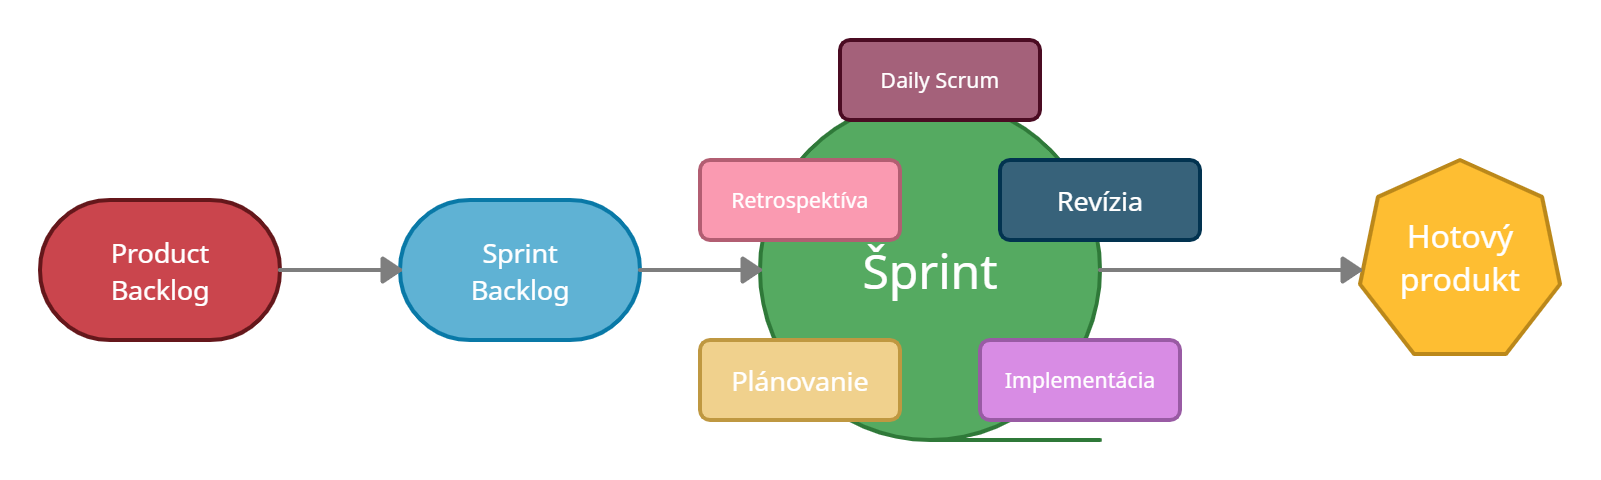
\includegraphics[width=1.0\textwidth]{diagram}
%Aj text môže byť prezentovaný ako obrázok. Stane sa z neho označný plávajúci objekt. Po vytvorení diagramu zrušte znak \texttt{\%} pred príkazom \verb|\includegraphics| označte tento riadok ako komentár (tiež pomocou znaku \texttt{\%}).
\caption{Náhodný obrázok.}
\label{f:rozhod}
\end{figure*}

\cite{agile}

\cite{techScrum}

\section{Funkcie v Scrume} \label{funkcie}

Scrum dodržiava špecifický spôsob rozdeľovania úloh pri vývoji projektov. Scrum Tím je tím všetkých účastníkov v Scrum procese, ktorý sa rozdeľuje na Scrum Mastera, Product Ownera a samotný Tím, teda tím developerov. Treba rozlišovať Tím a Scrum Tím, tieto pojmy sa často mýlia. Všetci účastníci Scrumu spolu blízko spolupracujú, komunikujú a riešia problémy. Snažia sa sústrediť sa vždy na jeden spoločný cieľ, ktorý sa v Scrume nazýva Product Goal. Scrum Tímy prirodzene fungujú lepšie, keď sú menšie, ľudia spolu vedia bližšie komunikovať a sú produktívnejší. Menej ľudí tak často spraví viac práce. Ukázalo sa, že najvýhodnejšie je mať v tíme 10 a menej ľudí. Vo veľkých spoločnostiach preto treba Scrum správne implementovať, čo vyžaduje skúsených manažérov.

\subsection{Scrum Master}

\subsection{Product Owner}

\subsection{Scrum Tím}

\section{Vývojový Proces} \label{proces}

\section{Výhody Scrumu} \label{proces}

\section{Záver} \label{zaver}




%\acknowledgement{Ak niekomu chcete poďakovať\ldots}


% týmto sa generuje zoznam literatúry z obsahu súboru literatura.bib podľa toho, na čo sa v článku odkazujete
\bibliography{literatura}
\bibliographystyle{alpha} % prípadne alpha, abbrv alebo hociktorý iný
\end{document}
